% Provenance (never printed): enseignement scientifique premiere (2019),
% "Le Soleil, notre source d'energie" (power received by latitude and
% season, albedo, the Earth's radiative balance, the small share stored by
% photosynthesis) and the old seconde/premiere S material on the
% atmosphere's energy; see sources/book2/PROVENANCE.md. Every insolation
% value, budget closure and photosynthesis figure is computed in
% figdata/grade-10/energy_budget.py; the budget fluxes are AR6 WG1
% Figure 7.2.
\chapter{Neraca Energi Bumi}\label{ch:g10:earth-energy-budget}

Pada hari terpanjang dalam setahun, Matahari sama sekali tidak terbenam di
Kutub Utara. Matahari mengitari langit sepanjang hari pada ketinggian yang
sama, sekitar \qty{23}{\degree} di atas cakrawala, dan puncak atmosfer di atas
kutub menerima dalam satu hari lebih banyak cahaya Matahari per meter persegi
daripada tempat mana pun di Bumi --- \qty{13.0}{kWh}, dibandingkan dengan
\qty{9.5}{kWh} di atas khatulistiwa. Namun laut di sekitar kutub tetap tertutup
es sepanjang musim panas. Sebaliknya, dalam setahun penuh, khatulistiwa
menerima cahaya Matahari dua setengah kali lebih banyak daripada kutub, dan
daerah tropis tetap hangat sepanjang tahun. Bab ini mengikuti energi cahaya
Matahari: berapa banyak yang datang, di mana, dan kapan; berapa banyak yang
langsung dipantulkan kembali ke angkasa; bagaimana sisanya dibagi antara udara
dan tanah, diangkut dari daerah tropis ke arah kutub, lalu akhirnya dikirim
kembali ke angkasa sebagai cahaya inframerah --- dan bagian kecil mana yang
akhirnya disimpan oleh makhluk hidup.
% ledger: earth:TSI, earth:obliquity (daily totals computed in figdata/grade-10/energy_budget.py)

\begin{omfigure}
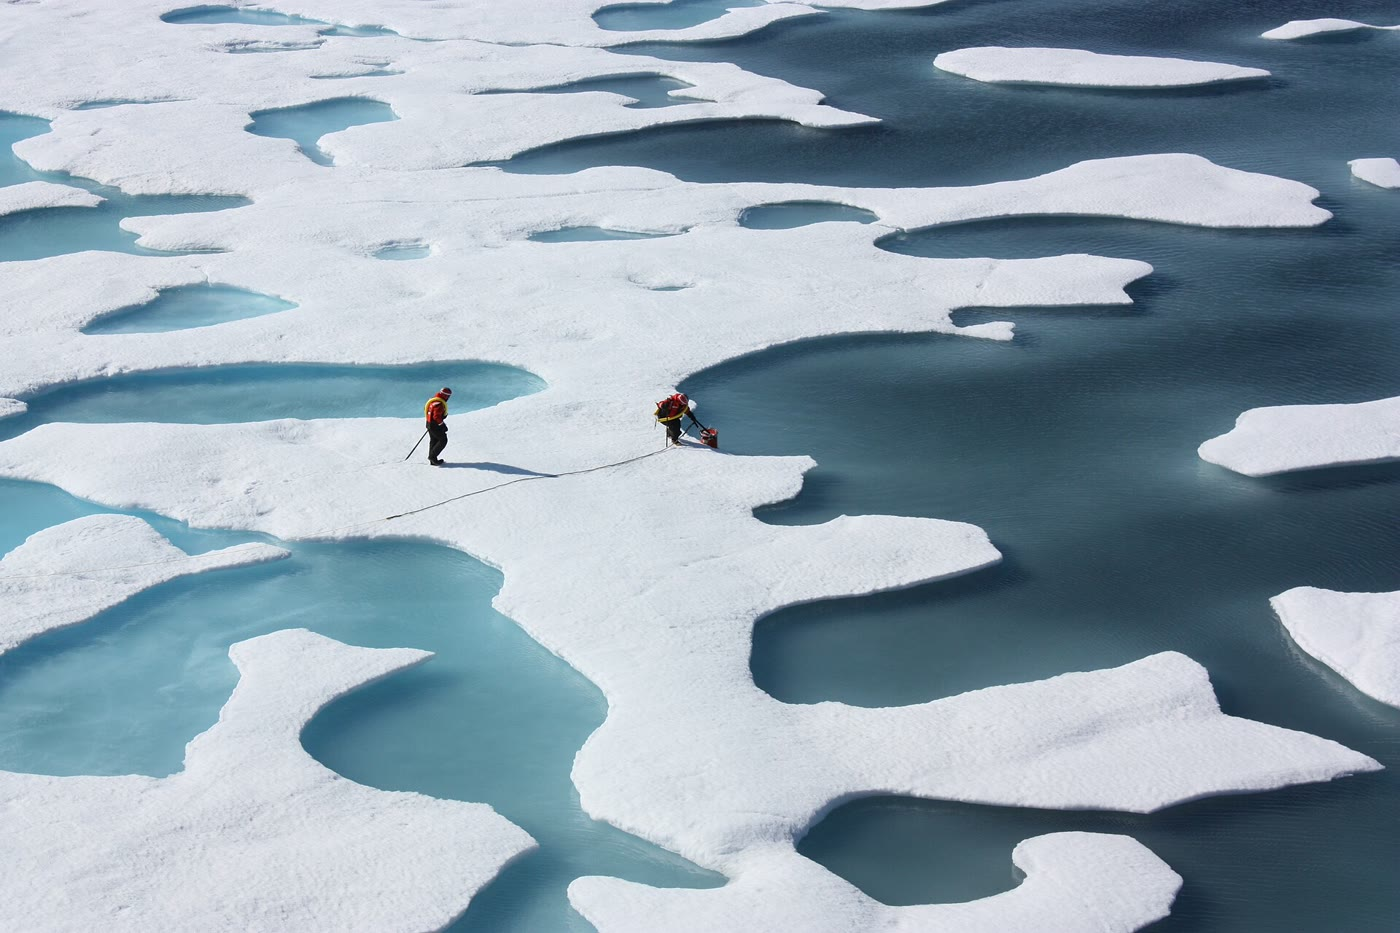
\includegraphics[width=0.78\linewidth]{images/book2/g10-nasa-melt-ponds.jpg}

{\small Es laut di Samudra Arktik pada bulan Juli, di bawah Matahari yang tidak
terbenam: es putih, kolam-kolam air lelehan di permukaannya, dan laut terbuka
yang gelap di antara bongkah-bongkah es. Dua ilmuwan mengambil sampel air
kolam. Foto: NASA Goddard Space Flight Center, 2011 (domain publik).}
\end{omfigure}

\begin{recall}
Musim-musim terjadi karena kemiringan sumbu Bumi, \qty{23.44}{\degree} dari
garis tegak lurus bidang orbitnya: pada bulan Juni belahan bumi utara condong
ke arah Matahari, yang naik lebih tinggi di langitnya dan bersinar lebih lama
(buku-buku fisika, dan Buku 1). Iradiansi pada jarak Bumi,
$S_0 = \qty{1361}{W/m^2}$, \omterm{def:g10:earth-energy-budget:albedo}{albedo} Bond sebuah planet, dan \omterm{def:g10:habitable-planet:equilibrium-temperature}{suhu
kesetimbangannya} sudah dibahas dalam \cref{ch:g10:habitable-planet}. Gas rumah
kaca menyerap sebagian inframerah yang dipancarkan permukaan (buku-buku kimia).
Udara hangat naik dan udara dingin turun, sehingga udara berputar dalam
sel-sel konveksi dan menggerakkan angin global (Buku 1, kelas 8). Tumbuhan,
alga, dan sebagian bakteri membuat gula dari karbon dioksida dan air dengan
energi cahaya: fotosintesis (buku-buku biologi).
\end{recall}

\section{Cahaya Matahari yang diterima}

Dilihat dari Matahari, Bumi tampak sebagai piringan. Setiap detik, Bumi
menangkap cahaya Matahari yang jatuh pada piringan berjari-jari $R$, yaitu
jari-jarinya sendiri; tetapi cahaya itu dibagi di antara semua titik sebuah
bola, yang separuhnya sedang mengalami malam.

\begin{proposition}[Seperempat tetapan Matahari]\label{prop:g10:earth-energy-budget:quarter}
Dirata-ratakan atas seluruh permukaan Bumi dan atas siang dan malam, daya
cahaya Matahari yang tiba di puncak atmosfer adalah
\[
  \frac{S_0}{4} = \frac{1361}{4} \approx \qty{340}{W/m^2}.
\]
\end{proposition}

\begin{proof}
Bumi menangkap cahaya Matahari yang melewati piringan seluas $\pi R^2$ yang
tegak lurus pada sinar, yaitu daya $S_0\,\pi R^2$. Bila disebarkan pada luas
bola, $4\pi R^2$, diperoleh $S_0\,\pi R^2/(4\pi R^2) =
S_0/4$ per meter persegi.
\end{proof}
% ledger: earth:TSI, ipcc:budget-toa

\begin{omfigure}
\begin{tikzpicture}[font=\small, >={Stealth[length=2mm]}]
  \foreach \y in {-1.2,-0.8,...,1.21}
    \draw[->, omProp!80!black] (-3.4,\y) -- (-1.75,\y);
  \node[anchor=south, font=\footnotesize, align=center] at (-2.6,1.35) {cahaya Matahari,\\$S_0$ per m$^2$};
  \draw[fill=omProp!15, draw=omProp!80!black] (-1.6,0) ellipse (0.18 and 1.3);
  \node[anchor=north, font=\footnotesize, align=center] at (-1.6,-1.4) {piringan\\$\pi R^2$};
  \shade[ball color=omDef!35] (1.2,0) circle (1.3);
  \fill[black, opacity=0.35] (1.2,1.3) arc (90:-90:1.3) arc (-90:90:0.35 and 1.3);
  \draw[omDef!80!black] (1.2,0) circle (1.3);
  \draw[dashed, black!50] (1.2,-1.3) arc (-90:90:0.35 and 1.3);
  \draw[<->] (1.2,0) -- node[above, font=\footnotesize] {$R$} (2.5,0);
  \node[anchor=west, font=\footnotesize, align=left] at (2.8,0.7) {bola $4\pi R^2$:\\separuh siang,\\separuh malam};
  \node[anchor=west, font=\footnotesize, align=left] at (2.8,-0.75) {rata-rata:\\$S_0\pi R^2/4\pi R^2 = S_0/4$};
\end{tikzpicture}

{\small Bumi menangkap cahaya Matahari yang jatuh pada piringan seukuran
jari-jarinya sendiri, tetapi membaginya pada luas bola yang empat kali lebih
besar: rata-rata, setiap meter persegi puncak atmosfer menerima seperempat
tetapan Matahari.}
\end{omfigure}

Rata-rata ini menyembunyikan perbedaan besar dari satu tempat ke tempat lain.
Berkas cahaya Matahari yang mengenai tanah secara miring tersebar pada luas
yang lebih besar daripada berkas yang mengenainya tegak lurus.

\begin{proposition}[Cahaya Matahari pada permukaan mendatar]\label{prop:g10:earth-energy-budget:height}
Bila Matahari berada pada ketinggian $h$ di atas cakrawala, satu meter persegi
mendatar di puncak atmosfer menerima daya $S_0 \sin h$.
\end{proposition}

\begin{proof}
Ambil berkas cahaya Matahari berpenampang persegi \qty{1}{m^2} yang membawa
$S_0$. Di tanah, jejaknya berupa persegi panjang yang satu sisinya \qty{1}{m}
dan sisi lainnya sepanjang $\ell$ searah kemiringan sinar. Dalam segitiga
siku-siku yang dibentuk oleh sisi itu, sinar, dan penampang berkas, sudut di
tanah adalah $h$ dan $\sin h = 1/\ell$. Daya berkas itu tersebar pada $\ell$
meter persegi: $S_0/\ell = S_0 \sin h$ per meter persegi.
\end{proof}

\begin{omfigure}
\begin{tikzpicture}[font=\small, >={Stealth[length=2mm]}]
  \fill[omExo!15] (-0.3,-0.5) rectangle (6.3,0);
  \draw[thick] (-0.3,0) -- (6.3,0);
  \foreach \s in {0,0.3,...,1.21}
    \draw[->, omProp!80!black] ({0.6+\s/sin(35)+3.2*cos(35)},{3.2*sin(35)}) -- ({0.6+\s/sin(35)+0.02*cos(35)},{0.02*sin(35)});
  \draw[omProp!80!black, thick] (0.6,0) -- ({0.6+1.2/sin(35)},0);
  \draw (0.6,0) ++(1.6,0) arc (0:35:1.6);
  \node[font=\footnotesize] at ({0.6+1.85*cos(17)},{1.85*sin(17)}) {$h$};
  \draw[<->] (0.6,-0.25) -- node[below, font=\footnotesize] {$\ell = 1/\sin h$} ({0.6+1.2/sin(35)},-0.25);
  \node[anchor=south west, font=\footnotesize, align=left] at (4.35,1.95) {berkas\\berpenampang\\\qty{1}{m^2}};
\end{tikzpicture}

{\small Cahaya Matahari yang tiba pada ketinggian $h$ di atas cakrawala:
berkas yang sama menutupi $1/\sin h$ meter persegi tanah mendatar, jadi setiap
meter persegi menerima $S_0 \sin h$. Makin rendah Matahari, makin lemah cahaya
Matahari di tanah.}
\end{omfigure}

Ketinggian Matahari berubah sepanjang hari, dan panjang hari berubah menurut
musim; keduanya ikut menentukan energi yang diterima suatu tempat.

\begin{definition}[Insolasi]\label{def:g10:earth-energy-budget:insolation}
Yang disebut \emph{insolasi}\index{insolasi} suatu tempat adalah daya cahaya
Matahari yang diterima satu meter persegi mendatar di puncak atmosfer di
atasnya. Dirata-ratakan atas dua puluh empat jam sehari, besaran itu disebut
\emph{insolasi rata-rata harian}; dirata-ratakan atas setahun, \emph{insolasi
rata-rata tahunan}; keduanya diukur dalam \unit{W/m^2}.
\end{definition}

Menghitung rata-rata harian memerlukan ketinggian Matahari pada setiap saat
sepanjang hari, yang memakai matematika di luar jangkauan buku ini; komputer
yang menggambar kurva di bawah ini sudah melakukannya. Ada dua kasus yang
sederhana. Di khatulistiwa pada saat ekuinoks, Matahari terbit tepat di timur,
melintas tepat di atas kepala pada tengah hari, dan terbenam tepat di barat
setelah dua belas jam; dirata-ratakan atas dua puluh empat jam, hasilnya
$S_0/\pi \approx \qty{433}{W/m^2}$ (diterima tanpa bukti). Di Kutub Utara,
Matahari hanya mengitari langit pada ketinggian tetap, dan contoh berikut
memakai hal itu.

\begin{example}[Kutub pada bulan Juni]\label{ex:g10:earth-energy-budget:pole}
% ledger: earth:TSI, earth:obliquity (values computed in figdata/grade-10/energy_budget.py)
Pada titik balik Juni, Matahari berada \qty{23.44}{\degree} di atas cakrawala
Kutub Utara sepanjang hari. \omterm{def:g10:earth-energy-budget:insolation}{Insolasi} rata-rata harian di sana adalah $1361
\times \sin 23.44^\circ \approx \qty{541}{W/m^2}$; selama dua puluh empat jam
nilainya $541 \times 24 \approx \qty{13000}{Wh}$, yaitu \qty{13.0}{kWh} per
meter persegi. Pada hari yang sama khatulistiwa menerima rata-rata harian
\qty{397}{W/m^2}, atau \qty{9.5}{kWh} per meter persegi: di sana Matahari naik
lebih tinggi pada tengah hari, tetapi berada di bawah cakrawala selama dua
belas jam.
\end{example}

\begin{omfigure}
\begin{tikzpicture}
\begin{axis}[omrecord, width=0.92\linewidth, height=6.4cm, xmin=1, xmax=365,
  ymin=0, ymax=600, ylabel={insolasi rata-rata harian (\unit{W/m^2})},
  xtick={1,32,60,91,121,152,182,213,244,274,305,335},
  xticklabels={J,F,M,A,M,J,J,A,S,O,N,D}, xlabel={bulan},
  legend style={at={(0.5,1.02)}, anchor=south, legend columns=4, font=\footnotesize, draw=none},
  tick label style={font=\small}, label style={font=\small}]
\addplot[omThm!85!black, thick] table[x=day, y=Q0] {figdata/out/grade-10-energy_budget-daily.dat};
\addlegendentry{khatulistiwa}
\addplot[omProp!90!black, thick, densely dashed] table[x=day, y=Q30] {figdata/out/grade-10-energy_budget-daily.dat};
\addlegendentry{\qty{30}{\degree} LU}
\addplot[omMeth!85!black, thick, dashdotted] table[x=day, y=Q60] {figdata/out/grade-10-energy_budget-daily.dat};
\addlegendentry{\qty{60}{\degree} LU}
\addplot[omDef!85!black, thick] table[x=day, y=Q90] {figdata/out/grade-10-energy_budget-daily.dat};
\addlegendentry{Kutub Utara}
\end{axis}
\end{tikzpicture}

{\small \omterm{def:g10:earth-energy-budget:insolation}{Insolasi} rata-rata harian di puncak atmosfer sepanjang tahun pada
empat lintang di belahan bumi utara (dihitung untuk orbit lingkaran, dari
tetapan Matahari dan kemiringan sumbu). Kutub tidak menerima apa pun selama
setengah tahun, dan menerima lebih banyak daripada tempat lain mana pun di
sekitar titik balik Juni.}
\end{omfigure}

\begin{remark}[Membaca kurva]\label{rem:g10:earth-energy-budget:curves}
\omterm{def:g10:earth-energy-budget:insolation}{Insolasi} khatulistiwa hampir tidak berubah: ada dua maksimum yang landai pada
saat ekuinoks, ketika Matahari melintas tepat di atas kepala pada tengah hari.
Makin jauh ke utara, makin besar ayunan antara musim panas dan musim dingin.
Di sebelah kutub dari $90^\circ - 23.44^\circ = \qty{66.56}{\degree}$,
Matahari tetap berada di bawah cakrawala pada titik balik Desember: itulah
malam kutub. Dari sekitar 10 Mei sampai akhir Juli, Kutub Utara dan lintang
\qty{60}{\degree} LU sama-sama menerima lebih banyak daripada khatulistiwa.
\end{remark}

Dalam setahun penuh gambarnya berubah: \omterm{def:g10:earth-energy-budget:insolation}{insolasi} rata-rata tahunan, yang
digambarkan pada subbab surplus dan defisit di bawah, turun dari \qty{416}{W/m^2} di khatulistiwa menjadi \qty{172}{W/m^2} di
kutub. Kelimpahan musim panas di daerah kutub tidak mengimbangi malamnya yang
panjang dan Mataharinya yang rendah.

\begin{remark}[Jarak ke Matahari tidak menyebabkan musim]\label{rem:g10:earth-energy-budget:distance}
% ledger: earth:peri, earth:aph, nasa:earth-perihelion-longitude (ratios computed)
Orbit Bumi tidak benar-benar berbentuk lingkaran: jaraknya ke Matahari berubah
antara \num{147.1} dan \num{152.1} juta kilometer, sekitar
\qty{3}{\percent}, sehingga cahaya Matahari berubah sekitar \qty{7}{\percent}.
Bumi paling dekat dengan Matahari pada awal Januari, di tengah musim dingin
belahan bumi utara. Kurva di atas mengabaikan perubahan kecil ini; musim
terjadi karena kemiringan sumbu, dan musim di kedua belahan bumi saling
berlawanan.
\end{remark}

\section{Albedo}

Sebagian cahaya Matahari yang sampai di Bumi tidak pernah menghangatkan apa
pun: awan, udara, salju, dan laut mengirimnya kembali ke angkasa.

\begin{definition}[Albedo]\label{def:g10:earth-energy-budget:albedo}
Yang disebut \emph{albedo}\index{albedo} sebuah permukaan adalah bagian cahaya
Matahari yang jatuh padanya yang dipantulkannya, yaitu bilangan antara 0
(seluruh cahaya diserap) dan 1 (seluruhnya dipantulkan). Albedo Bond dalam
\cref{ch:g10:habitable-planet} adalah albedo sebuah planet secara keseluruhan.
\end{definition}

\begin{omfigure}
\begin{tikzpicture}[font=\small, x=9cm, y=0.55cm]
  \foreach \lab/\lo/\hi/\n in {salju segar/0.80/0.90/8, es laut/0.50/0.70/7,
      pasir gurun/0.40/0.40/6, seluruh Bumi/0.30/0.30/5, rumput hijau/0.25/0.25/4,
      tanah gundul/0.17/0.17/3, hutan konifer/0.08/0.15/2, samudra terbuka/0.06/0.06/1,
      aspal baru/0.04/0.04/0} {
    \fill[omDef!45] (0,\n-0.32) rectangle (\lo,\n+0.32);
    \ifdim\hi pt>\lo pt
      \fill[omDef!18] (\lo,\n-0.32) rectangle (\hi,\n+0.32);
      \draw[omDef!80!black] (\lo,\n-0.32) rectangle (\hi,\n+0.32);
    \fi
    \draw[omDef!80!black] (0,\n-0.32) rectangle (\lo,\n+0.32);
    \node[anchor=east, font=\footnotesize] at (-0.01,\n) {\lab};
  }
  \draw (0,-0.6) -- (1,-0.6);
  \foreach \x in {0,0.2,...,1.01}
    \draw (\x,-0.6) -- (\x,-0.75) node[below, font=\footnotesize] {\pgfmathprintnumber[fixed, precision=1]{\x}};
  \node[font=\footnotesize] at (0.5,-2.0) {albedo};
\end{tikzpicture}

{\small \omterm{def:g10:earth-energy-budget:albedo}{Albedo} khas berbagai permukaan dan Bumi secara keseluruhan; bagian
batang yang pucat menunjukkan rentang yang biasa. Data: University of Colorado
Boulder, ekspedisi MOSAiC; National Snow and Ice Data Center.}
\end{omfigure}
% ledger: albedo:surfaces, nsidc:albedo-ice

Salju segar mengembalikan sebagian besar cahaya yang diterimanya, sedangkan
samudra terbuka hampir tidak mengembalikan apa pun. Itulah sebabnya es laut
pada foto pembuka tetap dingin sepanjang musim panas kutub: salju di atasnya
memantulkan sampai sembilan persepuluh cahaya Matahari, sedangkan air gelap di
antara bongkah-bongkah es menyerap sekitar 94 persen. Bila es mencair, air
gelap menggantikannya dan menyerap lebih banyak cahaya Matahari, yang
mencairkan lebih banyak es lagi: sebuah lingkaran yang saling memperkuat, yang
ditimbang oleh \cref{ch:g12:climate-change} di antara umpan balik iklim.

\begin{omfigure}
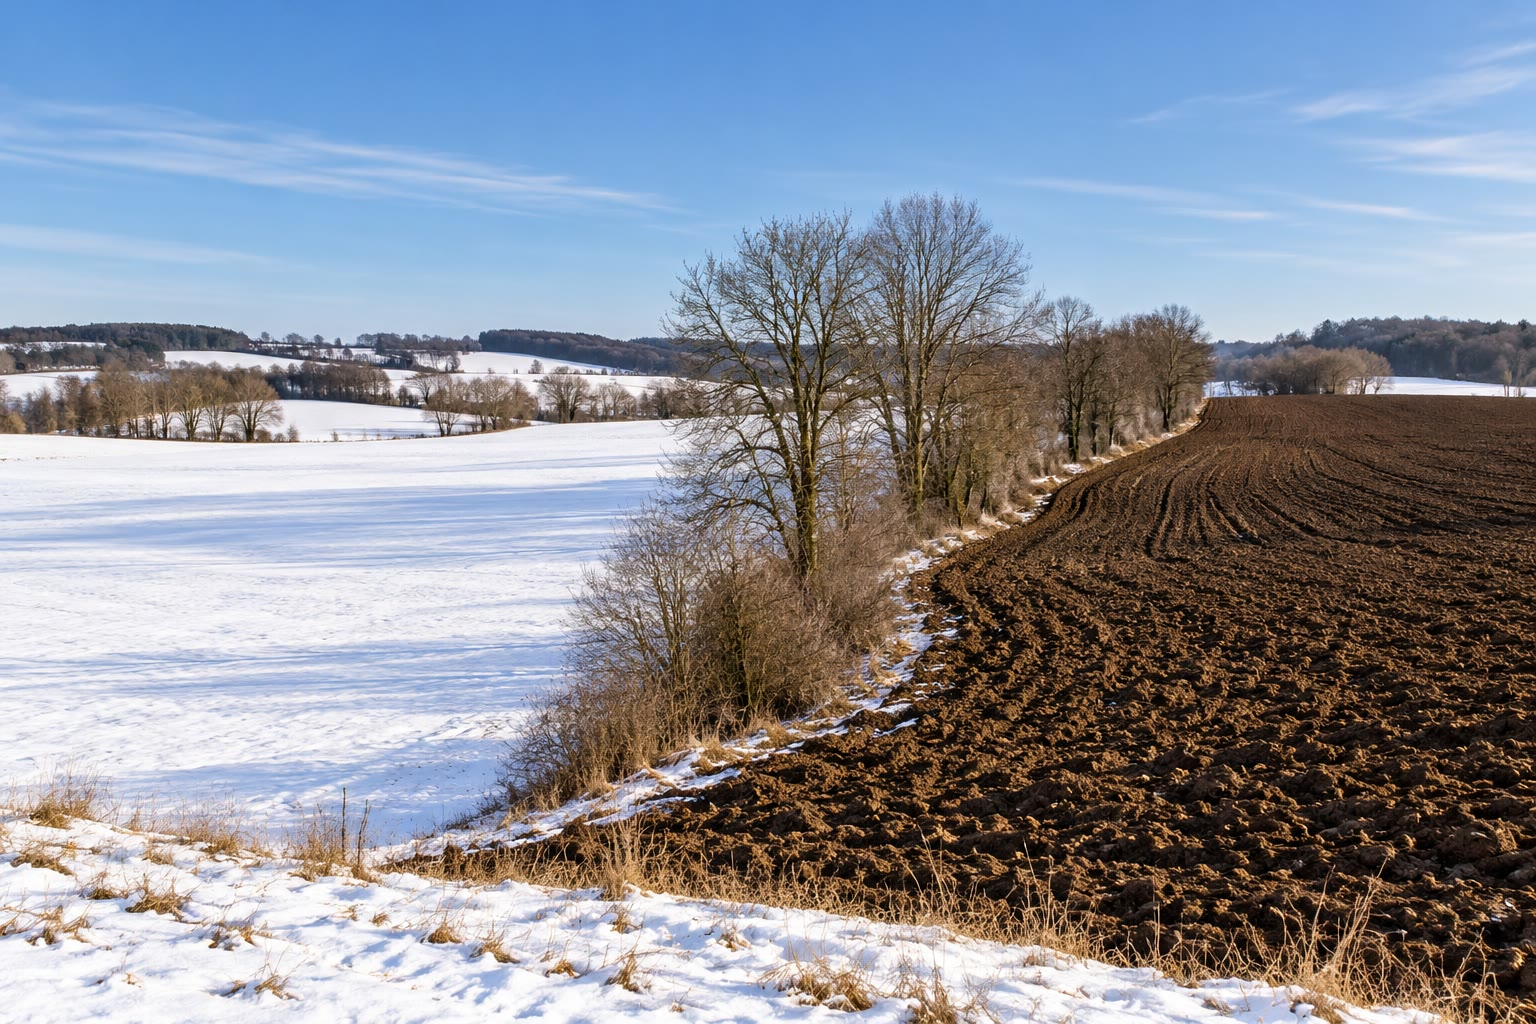
\includegraphics[width=0.7\linewidth]{images/book2/ai/g10-snow-and-ploughed-field.jpg}

{\small Pagi musim dingin setelah beberapa hari cerah: salju masih menutupi
padang rumput, tetapi sudah mencair di ladang gelap yang baru dibajak, yang
menyerap jauh lebih banyak cahaya Matahari.}
\end{omfigure}

Untuk Bumi secara keseluruhan, satelit mengukur langsung cahaya Matahari yang
dipantulkan ke angkasa: rata-rata \qty{100}{W/m^2} dari \qty{340}{W/m^2} yang
datang, yaitu \omterm{def:g10:earth-energy-budget:albedo}{albedo} $100/340 \approx 0.29$. Awan adalah pemantul utama:
pengukuran yang sama, dengan awan dihilangkan melalui perhitungan, hanya
memberikan \qty{53}{W/m^2} yang dipantulkan.
% ledger: ipcc:budget-toa, ipcc:budget-clearsky, earth:albedo

\begin{example}[Cahaya Matahari yang diserap Bumi]\label{ex:g10:earth-energy-budget:absorbed}
% ledger: earth:TSI, earth:albedo, earth:Rmean (computed in figdata/grade-10/energy_budget.py)
Dengan \omterm{def:g10:earth-energy-budget:albedo}{albedo} Bond 0.294, setiap meter persegi rata-rata menyerap $340
\times (1 - 0.294) \approx \qty{240}{W/m^2}$. Atas seluruh bola, yang luasnya
$4\pi R^2 = 4\pi \times (\qty{6.371e6}{m})^2 \approx \qty{5.10e14}{m^2}$, Bumi
menyerap $240 \times 5.10\times10^{14} \approx \qty{1.22e17}{W}$ cahaya
Matahari: daya inilah yang menggerakkan angin, arus laut, dan siklus air.
\end{example}

\section{Neraca energi global}

Ke mana perginya \qty{240}{W/m^2} ini? Pengukuran dari satelit, dari
instrumen di darat, dan dari kapal, yang digabungkan dengan model atmosfer,
kini memberikan jawaban yang konsisten, dirata-ratakan atas seluruh dunia dan
atas beberapa tahun. Kajian ilmiah tahun 2021 merangkumnya dalam diagram di
bawah ini, dan menyatakan bahwa komponen-komponen rata-rata global kini
diketahui dengan lebih akurat, di puncak atmosfer maupun di permukaan
(\emph{keyakinan tinggi}).
% ledger: ipcc:budget-confidence

\begin{definition}[Neraca energi]\label{def:g10:earth-energy-budget:energy-budget}
Yang disebut \emph{neraca energi}\index{neraca energi} sebuah sistem ---
seluruh Bumi, permukaannya, atau atmosfernya --- adalah perhitungan semua
energi yang masuk dan keluar dari sistem itu, dengan setiap aliran dinyatakan
sebagai daya rata-rata per meter persegi permukaan Bumi. Neraca itu
\emph{seimbang} bila yang masuk sama dengan yang keluar; jika tidak, sistem
itu memperoleh atau kehilangan energi, lalu menghangat atau mendingin.
\end{definition}

Permukaan juga kehilangan energi tanpa radiasi apa pun: air menguap dari laut
dan dari dedaunan, dan tanah menghangatkan udara yang bersentuhan dengannya.

\begin{definition}[Kalor laten; kalor sensibel]\label{def:g10:earth-energy-budget:latent-heat}
Yang disebut \emph{kalor laten}\index{kalor laten} suatu zat adalah energi
yang diserapnya ketika berubah wujud tanpa berubah suhu --- mencair, atau
menguap --- dan dilepaskannya kembali ketika kembali ke wujud semula. Untuk air
yang menguap pada \qty{15}{\degreeCelsius}, nilainya sekitar \qty{2.47}{MJ}
per kilogram. Dalam \omterm{def:g10:earth-energy-budget:energy-budget}{neraca energi}, \emph{fluks kalor laten} adalah energi yang
diambil penguapan dari permukaan dan yang dilepaskan uap air di udara tempat
uap itu mengembun menjadi awan. Fluks
\emph{kalor sensibel}\index{kalor sensibel} adalah energi yang diberikan permukaan kepada udara yang
bersentuhan dengannya, sehingga udara itu menghangat, dan yang diangkut ke
atas oleh udara yang naik.
\end{definition}
% ledger: nist:water-latent

\begin{omfigure}
\begin{tikzpicture}[font=\footnotesize, >={Stealth[length=2.2mm, width=2mm]}, line width=1.4pt]
  % layers
  \fill[omDef!8] (0,0.5) rectangle (12.8,4.5);
  \fill[omExo!35] (0,0) rectangle (12.8,0.5);
  \draw[thin, black!60] (0,0.5) -- (12.8,0.5);
  \draw[thin, black!60, dashed] (0,4.5) -- (12.8,4.5);
  \node[anchor=east, black!70, align=right] at (-0.1,5.4) {angkasa};
  \node[anchor=east, black!70, align=right] at (-0.1,4.5) {puncak\\atmosfer};
  \node[anchor=east, black!70, align=right] at (-0.1,2.5) {atmosfer};
  \node[anchor=east, black!70, align=right] at (-0.1,0.25) {permukaan};
  \pic[scale=0.7, transform shape] at (4.3,3.0) {puffycloud};
  \pic[scale=0.7, transform shape] at (6.2,3.0) {puffycloud};
  % sunlight
  \draw[->, omProp!90!black] (1.0,6.1) -- (1.0,0.52);
  \draw[->, omProp!90!black] (1.0,3.0) -- (1.6,3.0);
  \node[anchor=west, align=left] at (1.65,3.0) {80 diserap\\oleh udara};
  \node[anchor=west] at (1.05,1.3) {185};
  \draw[->, omProp!55] (4.3,3.7) -- (4.3,6.1);
  \node[anchor=east] at (4.25,5.0) {75};
  \draw[->, omProp!55] (5.25,0.52) -- (5.25,6.1);
  \node[anchor=west] at (5.3,1.2) {25};
  % heat
  \draw[->, omMeth!80!black] (6.2,0.52) -- (6.2,2.95);
  \draw[->, omMeth!80!black] (7.8,0.52) -- (7.8,2.0);
  % infrared
  \draw[->, omThm!80!black] (9.2,0.52) -- (9.2,4.0);
  \draw[->, omThm!80!black] (10.7,3.4) -- (10.7,6.1);
  \draw[->, omThm!50] (12.1,4.0) -- (12.1,0.52);
  % words above the top of the atmosphere
  \node[anchor=south, align=center] at (1.0,6.15) {340\\datang};
  \node[anchor=south, align=center] at (4.78,6.15) {100\\dipantulkan};
  \node[anchor=south, align=center] at (7.7,5.0) {ketidakseimbangan\\$+0.7$ diserap};
  \node[anchor=south, align=center] at (10.7,6.15) {239 inframerah\\ke angkasa};
  % words below the surface
  \node[anchor=north, align=center] at (1.0,-0.05) {160\\diserap};
  \node[anchor=north, align=center] at (6.2,-0.05) {82\\kalor\\laten};
  \node[anchor=north, align=center] at (7.8,-0.05) {21\\kalor\\sensibel};
  \node[anchor=north, align=center] at (9.4,-0.05) {398\\dipancarkan};
  \node[anchor=north, align=center] at (12.1,-0.05) {342\\radiasi\\balik};
\end{tikzpicture}

{\small \omterm{def:g10:earth-energy-budget:energy-budget}{Neraca energi} rata-rata global Bumi pada awal abad ke-21, dalam
\unit{W/m^2} yang dirata-ratakan atas seluruh permukaan. Jingga: cahaya
Matahari; hijau: kalor yang diangkut oleh penguapan dan oleh udara hangat;
merah: inframerah. Dari 100 yang dipantulkan, 25 berasal dari permukaan dan 75
dari awan, udara, dan debunya. Inframerah ke angkasa mencakup bagian pancaran
permukaan yang lolos langsung menembus udara. Data: IPCC, Laporan Penilaian
Keenam, Kelompok Kerja~I, Gambar~7.2.}
\end{omfigure}
% ledger: ipcc:budget-toa, ipcc:budget-surface

\begin{method}[Membaca diagram neraca energi]\label{met:g10:earth-energy-budget:reading}
\begin{enumerate}
  \item Pilih sistemnya: seluruh Bumi (garis di atas atmosfer), permukaan,
        atau atmosfer (lapisan di antara keduanya).
  \item Daftarlah panah-panah yang masuk ke sistem itu dan jumlahkan; daftarlah
        panah-panah yang keluar dan jumlahkan.
  \item Bandingkan kedua jumlah itu. Jika keduanya sama dalam batas pembulatan
        angka-angkanya, sistem itu seimbang; selisihnya adalah apa yang
        diperoleh (atau hilang) dari sistem itu setiap detik per meter
        persegi.
\end{enumerate}
\end{method}

\begin{proposition}[Neraca itu seimbang]\label{prop:g10:earth-energy-budget:balance}
Dalam batas pembulatan angka-angkanya, neraca pada diagram di atas seimbang
untuk Bumi secara keseluruhan, untuk permukaan, dan untuk atmosfer, kecuali
surplus kecil sekitar \qty{0.7}{W/m^2} yang diserap Bumi dan tidak
dikembalikannya.
\end{proposition}

\begin{proof}
\emph{Seluruh Bumi:} masuk, 340; keluar, $100 + 239 = 339$.
\emph{Permukaan:} masuk, $160 + 342 = 502$; keluar, $82 + 21 + 398 = 501$.
Dalam kedua kasus, surplusnya, sekitar 1, adalah ketidakseimbangan 0.7 yang
dibulatkan. \emph{Atmosfer:} sebut $W$ bagian inframerah permukaan yang lolos
menembus udara ke angkasa. Udara menerima $80 + 82 + 21 + (398 - W) = 581 - W$
dan memancarkan $342$ ke bawah dan $239 - W$ ke atas, seluruhnya $581 - W$:
seimbang, berapa pun $W$.
\end{proof}
% ledger: ipcc:budget-toa, ipcc:budget-surface (closures checked in figdata/grade-10/energy_budget.py)

Diagram itu juga memperlihatkan efek rumah kaca yang sedang bekerja.
Permukaan menerima dari udara, sebagai inframerah, \qty{342}{W/m^2} --- lebih
dari dua kali cahaya Matahari yang diserapnya, \qty{160}{W/m^2}. Itulah
sebabnya permukaan dapat memancarkan \qty{398}{W/m^2}, yaitu pancaran benda
bersuhu sekitar \qty{15}{\degreeCelsius}, sementara Bumi hanya mengirim
\qty{239}{W/m^2} ke angkasa. Buku-buku fisika membangun model yang
menghubungkan angka-angka ini dengan suhu; buku ini memakai fluks-fluks yang
terukur.

\begin{example}[Satu meter air setahun]\label{ex:g10:earth-energy-budget:evaporation}
% ledger: ipcc:budget-surface, nist:water-latent (computed in figdata/grade-10/energy_budget.py)
Fluks \omterm{def:g10:earth-energy-budget:latent-heat}{kalor laten}, \qty{82}{W/m^2}, setiap detik menguapkan $82/2.47\times
10^6 \approx \qty{3.3e-5}{kg}$ air per meter persegi. Dalam setahun,
$3.16\times10^7$ detik, jumlahnya sekitar \qty{1050}{kg}, yaitu lapisan air
setebal \qty{1.05}{m} di seluruh Bumi. Udara hanya menampung sedikit air pada
satu waktu, jadi hampir semuanya jatuh kembali sebagai hujan dan salju: fluks
\omterm{def:g10:earth-energy-budget:latent-heat}{kalor laten} dan curah hujan tahunan planet ini adalah dua sisi dari siklus air
yang sama.
\end{example}

\begin{remark}[Ketidakseimbangan]\label{rem:g10:earth-energy-budget:imbalance}
% ledger: ipcc:budget-toa, ipcc:heating
Surplus sebesar \qty{0.7}{W/m^2} tampak sangat kecil dibandingkan dengan fluks
yang ratusan watt, tetapi atas seluruh Bumi nilainya $0.7 \times 5.10\times10^{14} \approx
\qty{3.6e14}{W}$, yang sebagian besar tersimpan di
samudra, yang menjadi makin hangat. Ketidakseimbangan itu bukan tetapan alam:
nilainya bertambah dalam beberapa dasawarsa terakhir, seperti dijelaskan
\cref{ch:g12:climate-change}.
\end{remark}

\section{Surplus dan defisit}

Neraca itu seimbang untuk Bumi secara keseluruhan, tetapi tidak pada setiap lintang.

\begin{omfigure}
\begin{tikzpicture}
\begin{axis}[omrecord, width=0.86\linewidth, height=5.6cm, xmin=0, xmax=90,
  ymin=0, ymax=450, xlabel={lintang (\unit{\degree})},
  ylabel={insolasi rata-rata tahunan (\unit{W/m^2})}, xtick={0,15,...,90},
  tick label style={font=\small}, label style={font=\small}]
\addplot[omThm!85!black, thick] table[x=lat, y=Qann] {figdata/out/grade-10-energy_budget-annual.dat};
\addplot[omDef!80!black, dashed, domain=0:90] {340.25};
\node[anchor=south west, font=\footnotesize, omDef!80!black] at (axis cs:2,343) {rata-rata global, 340};
\node[anchor=south west, font=\footnotesize, omThm!85!black] at (axis cs:62,232) {rata-rata tahunan};
\end{axis}
\end{tikzpicture}

{\small \omterm{def:g10:earth-energy-budget:insolation}{Insolasi} rata-rata tahunan di puncak atmosfer terhadap lintang (sama di
kedua belahan bumi; dihitung dari tetapan Matahari dan kemiringan sumbu). Di
antara khatulistiwa dan sekitar \qty{37}{\degree}, nilainya melebihi rata-rata
global; ke arah kutub dari lintang itu nilainya kurang.}
\end{omfigure}

Daerah tropis menyerap jauh lebih banyak cahaya Matahari daripada daerah
kutub, dan \omterm{def:g10:earth-energy-budget:albedo}{albedonya} yang rendah memperlebar selisih itu. Inframerah yang
dikirimnya ke angkasa juga lebih besar, karena daerah tropis lebih hangat,
tetapi besarnya jauh kurang berubah terhadap lintang. Akibatnya, daerah di
sekitar khatulistiwa rata-rata menyerap sekitar \qty{200}{W/m^2} lebih banyak
daripada yang dipantulkan dan dipancarkannya, sedangkan daerah di dekat kutub
memancarkan sekitar \qty{200}{W/m^2} lebih banyak daripada yang diserapnya.
% ledger: nasaeo:surplus

\begin{definition}[Transpor kalor ke arah kutub]\label{def:g10:earth-energy-budget:heat-transport}
Yang disebut
\emph{transpor kalor ke arah kutub}\index{transpor kalor ke arah kutub} adalah aliran energi yang diangkut dari daerah tropis ke arah kutub oleh
gerakan atmosfer dan samudra. Besarnya diukur melintasi sebuah lingkaran
lintang, dalam petawatt (\qty{1}{PW} = \qty{e15}{W}).
\end{definition}

Tanpa transpor itu, daerah tropis akan makin panas dan daerah kutub makin
dingin sampai setiap lintang menyeimbangkan neracanya sendiri. Atmosfer
melakukan sebagian besar pengangkutan: udara hangat bergerak ke arah kutub dan
udara dingin kembali ke arah khatulistiwa, sedangkan uap air melepaskan \omterm{def:g10:earth-energy-budget:latent-heat}{kalor
latennya} jauh dari tempat air itu menguap. Arus laut mengangkut sisanya.
Perkiraan dari pengukuran menempatkan transpor atmosfer ke arah kutub pada
maksimum sekitar \qty{5.0}{PW} di dekat \qty{43}{\degree} LU, dengan nilai
serupa di dekat \qty{40}{\degree} LS; samudra mengangkut lebih banyak daripada
atmosfer hanya di dekat khatulistiwa, antara \qty{0}{\degree} dan
\qty{17}{\degree} LU, dan pada \qty{35}{\degree} LU, tempat transpor total
paling besar, atmosfer mengangkut \qty{78}{\percent} di antaranya. Transpor
total paling besar di sana karena \qty{35}{\degree} kira-kira merupakan tempat
surplus berganti menjadi defisit: ke arah khatulistiwa, transpor itu terus
mengumpulkan surplus setiap lintang yang dilintasinya; ke arah kutub, setiap
lintang mengambil darinya.
% ledger: trenberth:transport

\begin{omfigure}
\begin{tikzpicture}[font=\footnotesize, >={Stealth[length=2mm]}]
  \def\R{2.4}
  \begin{scope}
    \clip (0,0) circle (\R);
    \fill[omThm!22] (-\R,{-\R*sin(35)}) rectangle (\R,{\R*sin(35)});
    \fill[omDef!22] (-\R,{\R*sin(35)}) rectangle (\R,\R);
    \fill[omDef!22] (-\R,-\R) rectangle (\R,{-\R*sin(35)});
  \end{scope}
  \draw[thick] (0,0) circle (\R);
  \draw[black!50] (-\R,0) -- (\R,0);
  \foreach \s in {1,-1} \draw[black!40, dashed] ({-\R*cos(35)},{\s*\R*sin(35)}) -- ({\R*cos(35)},{\s*\R*sin(35)});
  \node at (0,0.45) {surplus};
  \node at (0,1.95) {defisit};
  \node at (0,-1.95) {defisit};
  \node[anchor=west, black!60] at (\R+0.05,0) {khatulistiwa};
  \node[anchor=west, black!60] at ({\R*cos(35)+0.05},{\R*sin(35)}) {\qty{35}{\degree} LU};
  \node[anchor=west, black!60] at ({\R*cos(35)+0.05},{-\R*sin(35)}) {\qty{35}{\degree} LS};
  \foreach \s in {1,-1} {
    \draw[->, very thick, omProp!90!black] ({-(\R+0.35)*cos(10)},{\s*(\R+0.35)*sin(10)}) arc ({180-10*\s}:{180-70*\s}:{\R+0.35});
    \draw[->, thick, omMeth!80!black] ({-(\R-0.45)*cos(8)},{\s*(\R-0.45)*sin(8)}) arc ({180-8*\s}:{180-55*\s}:{\R-0.45});
  }
  \node[anchor=east, omProp!90!black, align=right] at (-\R-0.75,1.6) {atmosfer};
  \node[anchor=east, omProp!90!black, align=right] at (-\R-0.75,-1.6) {atmosfer};
  \node[omMeth!80!black] at (-1.25,0.62) {samudra};
  \node[omMeth!80!black] at (-1.25,-0.62) {samudra};
\end{tikzpicture}

{\small Di antara sekitar \qty{35}{\degree} LS dan \qty{35}{\degree} LU Bumi
menyerap lebih banyak energi daripada yang dipancarkannya; ke arah kutub dari
lintang-lintang itu, Bumi memancarkan lebih banyak daripada yang diserapnya.
Atmosfer (jingga) dan samudra (hijau) mengangkut surplus itu ke arah kutub.
Skema: lebar panah tidak berskala.}
\end{omfigure}

Transpor inilah mesin cuaca. Sel-sel konveksi dan angin global dalam Buku 1,
badai dalam \cref{ch:g10:storms-and-cyclones}, dan arus-arus laut besar dalam
\cref{ch:g10:layered-ocean} semuanya memindahkan kalor dari tempat Matahari
memberi terlalu banyak ke tempat Matahari memberi terlalu sedikit.

\section{Ke mana energi itu pergi}

Hampir seluruh energi cahaya Matahari yang diserap Bumi akhirnya menjadi
kalor: energi itu menghangatkan tanah, laut, dan udara, menguapkan air,
menggerakkan angin dan arus, lalu pergi lagi sebagai cahaya inframerah.
Sebagian kecil menempuh jalan lain: fotosintesis menyimpannya dalam ikatan
kimia gula, dan dari situ dalam seluruh materi hidup di planet ini.

\begin{example}[Bagian fotosintesis]\label{ex:g10:earth-energy-budget:photosynthesis}
% ledger: field:npp, nist:glucose-combustion, earth:Rmean (computed in figdata/grade-10/energy_budget.py)
Tumbuhan di darat dan alga di laut, setelah memenuhi kebutuhannya sendiri,
menyimpan sekitar \num{105} miliar ton karbon dalam materi hidup baru setiap
tahun, kira-kira separuh di darat dan separuh di samudra: para ahli ekologi
menyebutnya produksi primer bersih planet ini. Membakar satu mol glukosa,
\ce{C6H12O6}, yang mengandung enam mol karbon, \qty{72}{g}, melepaskan
\qty{2805}{kJ}: sekitar \qty{38.9}{kJ} per gram karbon. Energi yang disimpan
setiap tahun adalah $1.049\times10^{17}\,\unit{g} \times \qty{38.9e3}{J/g} \approx
\qty{4.1e21}{J}$, yaitu daya sebesar $4.1\times10^{21}/3.16\times10^{7} \approx
\qty{1.3e14}{W}$. Dibandingkan dengan \qty{1.22e17}{W} cahaya Matahari yang
diserap Bumi, nilai ini sekitar \qty{0.1}{\percent}.
\end{example}

\begin{remark}[Bagian yang kecil, peran yang besar]\label{rem:g10:earth-energy-budget:life}
Seperseribu cahaya Matahari yang diserap menghidupi hampir seluruh kehidupan
di Bumi, dan sisa-sisa tumbuhan dan alga yang terkubur selama ratusan juta
tahun membentuk batu bara, minyak bumi, dan gas alam
(\cref{ch:g11:fossil-fuel-geology}). Sisa cahaya Matahari --- lebih dari 99.9
persen --- menjaga planet ini tetap hangat serta udara, air, dan cuacanya
tetap bergerak.
\end{remark}

\section{Latihan}

\begin{exercise}[$\star$]\label{exo:g10:earth-energy-budget:1}
Definisikan \omterm{def:g10:earth-energy-budget:insolation}{insolasi} suatu tempat dan \omterm{def:g10:earth-energy-budget:albedo}{albedo} sebuah permukaan. Manakah yang
memantulkan bagian cahaya Matahari yang lebih besar, salju segar atau samudra
terbuka?
\end{exercise}

\begin{exercise}[$\star$]\label{exo:g10:earth-energy-budget:2}
Dengan diagram \omterm{def:g10:earth-energy-budget:energy-budget}{neraca energi} dalam bab ini, nyatakan sebagai persentase dari
\qty{340}{W/m^2} yang tiba di puncak atmosfer bagian yang dipantulkan ke
angkasa, bagian yang diserap udara, dan bagian yang diserap permukaan.
\end{exercise}

\begin{exercise}[$\star$]\label{exo:g10:earth-energy-budget:3}
Matahari musim panas menyalurkan \qty{800}{W/m^2} ke tanah. Berapa daya yang
diserap satu meter persegi jika tertutup aspal baru (\omterm{def:g10:earth-energy-budget:albedo}{albedo} 0.04), dan jika
tertutup salju segar (\omterm{def:g10:earth-energy-budget:albedo}{albedo} 0.85)?
\end{exercise}

\begin{exercise}[$\star$]\label{exo:g10:earth-energy-budget:4}
Manakah yang mengangkut lebih banyak energi dari permukaan Bumi, penguapan
atau pemanasan udara yang bersentuhan dengan tanah? Uraikan dalam dua kalimat
bagaimana energi yang diambil penguapan dari laut sampai di udara jauh di
atasnya.
\end{exercise}

\begin{exercise}[$\star$]\label{exo:g10:earth-energy-budget:5}
Jelaskan mengapa \omterm{def:g10:earth-energy-budget:insolation}{insolasi} rata-rata harian di Kutub Utara bernilai nol pada
bulan Desember, dan sebutkan lintang yang di atasnya hal ini terjadi pada
titik balik Desember.
\end{exercise}

\begin{exercise}[$\star\star$]\label{exo:g10:earth-energy-budget:6}
Dengan \cref{prop:g10:earth-energy-budget:height}, hitung daya yang diterima
satu meter persegi mendatar di puncak atmosfer bila Matahari berada
\qty{90}{\degree}, \qty{30}{\degree}, dan \qty{10}{\degree} di atas
cakrawala. Pada ketinggian Matahari berapa meter persegi itu menerima setengah
$S_0$?
\end{exercise}

\begin{exercise}[$\star\star$]\label{exo:g10:earth-energy-budget:7}
Dengan mengikuti \cref{met:g10:earth-energy-budget:reading}, periksa neraca
cahaya Matahari saja: dari \qty{340}{W/m^2} yang tiba, berapa yang
dipantulkan, diserap udara, dan diserap permukaan? Apakah jumlah ketiganya
340? Periksa juga bahwa cahaya Matahari yang sampai di permukaan,
\qty{185}{W/m^2}, dipantulkan atau diserap di sana.
\end{exercise}

\begin{exercise}[$\star\star$]\label{exo:g10:earth-energy-budget:8}
Dengan jari-jari rata-rata Bumi \qty{6371}{km}, hitung luas piringan yang
menangkap cahaya Matahari dan daya yang ditangkapnya, lalu luas bola.
Simpulkan daya rata-rata per meter persegi bola.
\end{exercise}

\begin{exercise}[$\star\star$]\label{exo:g10:earth-energy-budget:9}
Surplus Bumi adalah \qty{0.7}{W/m^2} pada luas \qty{5.10e14}{m^2}. Berapa
energi, dalam joule, yang diperoleh Bumi dalam setahun yang lamanya
$3.16\times10^7$ detik?
\end{exercise}

\begin{exercise}[$\star\star$]\label{exo:g10:earth-energy-budget:10}
Jika awan dihilangkan melalui perhitungan, Bumi akan memantulkan
\qty{53}{W/m^2}, bukan \qty{100}{W/m^2}, dan mengirim \qty{267}{W/m^2}
inframerah ke angkasa, bukan \qty{239}{W/m^2}. Berapa besar awan mengubah
cahaya Matahari yang diserap, dan inframerah yang hilang? Secara keseluruhan,
apakah awan menghangatkan atau mendinginkan Bumi?
\end{exercise}

\begin{exercise}[$\star\star$]\label{exo:g10:earth-energy-budget:11}
Bacalah kurva \omterm{def:g10:earth-energy-budget:insolation}{insolasi} rata-rata harian dalam bab ini. Pada bulan apa saja
\omterm{def:g10:earth-energy-budget:insolation}{insolasi} rata-rata harian di Kutub Utara lebih besar daripada di khatulistiwa?
Mengapa kurva khatulistiwa menunjukkan dua maksimum, bukan satu?
\end{exercise}

\begin{exercise}[$\star\star\star$]\label{exo:g10:earth-energy-budget:12}
\omterm{def:g10:earth-energy-budget:latent-heat}{Kalor laten} penguapan air adalah \qty{2.47}{MJ/kg} dan fluks \omterm{def:g10:earth-energy-budget:latent-heat}{kalor laten}
\qty{82}{W/m^2}. Hitung tebal air, dalam milimeter, yang diuapkan dari satu
meter persegi rata-rata Bumi setiap hari, dan dalam meter setiap tahun (satu
liter air yang disebarkan pada satu meter persegi membentuk lapisan setebal
\qty{1}{mm}).
\end{exercise}

\begin{exercise}[$\star\star\star$]\label{exo:g10:earth-energy-budget:13}
Di Kutub Utara Matahari mengitari langit pada ketinggian yang sama dengan
deklinasinya $\delta$, jadi \omterm{def:g10:earth-energy-budget:insolation}{insolasi} rata-rata harian di sana adalah $S_0 \sin
\delta$. Tentukan deklinasi yang membuat kutub menerima, rata-rata dalam
sehari, sama banyaknya dengan khatulistiwa pada saat ekuinoks, $S_0/\pi$.
Deklinasi memenuhi $\sin\delta = \sin 23.44^\circ \times \sin\lambda$, dengan
sudut $\lambda$ yang bertambah secara teratur sebesar \qty{360}{\degree} dalam
setahun, dari \qty{0}{\degree} pada ekuinoks Maret (\qty{90}{\degree} pada
titik balik Juni). Kira-kira berapa hari dalam setahun kutub menerima lebih
dari $S_0/\pi$?
\end{exercise}

\begin{exercise}[$\star\star\star$]\label{exo:g10:earth-energy-budget:14}
Andaikan pada musim panas es laut seluas \qty{1e12}{m^2} (\omterm{def:g10:earth-energy-budget:albedo}{albedo} 0.6) mencair
dan digantikan oleh samudra terbuka (\omterm{def:g10:earth-energy-budget:albedo}{albedo} 0.06), di bawah cahaya Matahari
yang rata-rata \qty{300}{W/m^2} di permukaan. Hitung daya tambahan yang
diserap. Bandingkan dengan daya yang disimpan oleh seluruh fotosintesis di
Bumi, \qty{1.3e14}{W}, dan jelaskan mengapa pertukaran permukaan ini
memperkuat dirinya sendiri.
\end{exercise}

\begin{exercise}[$\star\star\star$]\label{exo:g10:earth-energy-budget:15}
Jarak Bumi ke Matahari adalah \num{147.1} juta kilometer pada titik
terdekatnya dan \num{152.1} juta pada titik terjauhnya, dengan rata-rata
\num{149.6} juta, tempat $S_0 = \qty{1361}{W/m^2}$. Hitung iradiansi Matahari
pada kedua titik ekstrem itu. Selisihnya mendekati \qty{90}{W/m^2}; pada
\qty{60}{\degree} LU, \omterm{def:g10:earth-energy-budget:insolation}{insolasi} rata-rata harian sekitar \qty{490}{W/m^2} pada
bulan Juni dan \qty{24}{W/m^2} pada bulan Desember. Jelaskan mengapa jarak
tidak mungkin menjadi penyebab musim.
\end{exercise}

\section{Soal: Mengikuti Seberkas Cahaya Matahari}

\begin{problem}[{Soal akhir pekan --- dari cahaya Matahari yang sampai di Bumi
sampai bagian yang disimpan kehidupan}]
\label{pb:g10:earth-energy-budget:1}
% ledger: earth:TSI, earth:Rmean, ipcc:budget-toa, ipcc:budget-surface, ipcc:budget-clearsky, nist:water-latent, field:npp, nist:glucose-combustion (all results computed in figdata/grade-10/energy_budget.py or from the rounded data below)
Gunakan $S_0 = \qty{1361}{W/m^2}$, jari-jari Bumi $R = \qty{6371}{km}$,
$\sigma = \qty{5.67e-8}{W.m^{-2}.K^{-4}}$, satu tahun $3.156\times10^7$
detik, fluks-fluks pada diagram \omterm{def:g10:earth-energy-budget:energy-budget}{neraca energi}, \omterm{def:g10:earth-energy-budget:latent-heat}{kalor laten} penguapan
\qty{2.47}{MJ/kg}, produksi primer bersih global \num{104.9} miliar ton
karbon per tahun, dan \qty{2805}{kJ} yang dilepaskan pembakaran satu mol
glukosa (\qty{72.07}{g} karbon).

\medskip
\noindent\textbf{Bagian I --- Geometri cahaya Matahari.}
\begin{enumerate}
  \item Hitung luas piringan yang menangkap cahaya Matahari, $\pi R^2$, dalam
        meter persegi.
  \item Hitung daya cahaya Matahari yang ditangkapnya.
  \item Hitung luas permukaan Bumi, $4\pi R^2$.
  \item Simpulkan daya rata-rata yang tiba per meter persegi puncak
        atmosfer.
  \item Pada saat ekuinoks pada tengah hari, Matahari berada tepat di atas
        kepala di khatulistiwa dan \qty{30}{\degree} di atas cakrawala pada
        \qty{60}{\degree} LU. Berapa daya yang diterima satu meter persegi
        mendatar di setiap tempat?
\end{enumerate}

\medskip
\noindent\textbf{Bagian II --- Albedo.}
\begin{enumerate}[resume]
  \item Dari \qty{100}{W/m^2} yang dipantulkan, hitung \omterm{def:g10:earth-energy-budget:albedo}{albedo} Bumi.
  \item Hitung daya yang diserap per meter persegi dan oleh seluruh Bumi.
  \item Tanpa awan, \qty{53}{W/m^2} akan dipantulkan. Berapa \omterm{def:g10:earth-energy-budget:albedo}{albedonya}? Dengan
        faktor berapa awan menaikkannya?
  \item Hitung \omterm{def:g10:habitable-planet:equilibrium-temperature}{suhu kesetimbangan} yang sesuai dengan daya yang diserap pada
        pertanyaan 7 (\cref{ch:g10:habitable-planet}), dan bandingkan dengan
        \qty{288}{K} permukaan.
\end{enumerate}

\medskip
\noindent\textbf{Bagian III --- Permukaan.}
\begin{enumerate}[resume]
  \item Jumlahkan aliran-aliran energi yang masuk ke permukaan.
  \item Jumlahkan aliran-aliran yang keluar, lalu bandingkan.
  \item Berapa kali lebih besar inframerah yang diterima permukaan dari udara
        dibandingkan dengan cahaya Matahari yang diserapnya? Apa yang
        ditunjukkan hal ini?
  \item Hitung massa air yang diuapkan dari satu meter persegi dalam setahun,
        dan tebal lapisan yang dibentuknya.
  \item Hitung daya total ketidakseimbangan, \qty{0.7}{W/m^2}, atas seluruh
        Bumi.
\end{enumerate}

\medskip
\noindent\textbf{Bagian IV --- Bagian kehidupan.}
\begin{enumerate}[resume]
  \item Hitung energi yang disimpan per gram karbon yang diikat dalam glukosa.
  \item Hitung energi yang disimpan dalam setahun oleh produksi primer bersih.
  \item Ubahlah energi itu menjadi daya.
  \item Nyatakan daya itu per meter persegi permukaan Bumi.
  \item Bandingkan dengan ketidakseimbangan pada pertanyaan 14.
  \item Berapa bagian cahaya Matahari yang diserap Bumi (pertanyaan 7) yang
        disimpan oleh fotosintesis?
\end{enumerate}
\end{problem}
